% !TEX root = main.tex
\setmathfont[Scale=MatchUppercase]{XITS Math}
\chapter[head={\CP violation in the $B$ meson sector},tocentry={$\symbfsf{C{}P}$ violation in the $\symbfsf{B}$ meson sector}]
{$\symbfsf{C{}P}$ violation in the $\symbfsf{B}$ meson sector}
\label{chap:CPV}
\setmathfont{Tex Gyre Pagella Math}

\linespread{1.08}\selectfont
Since in the \ac{SM}, all physical interactions are conserved under the $CPT$ transformation, the violation of \CP is equivalent to a violation of the $T$ symmetry.
As described in \cref{sec:symmetriesInSM}, the $T$ operator is antiunitary and it therefore transforms numbers into their complex conjugate.
Hence, \CP transformations only affect the complex phases of the wave functions describing initial and final states.
However, the absolute values of phases describing transitions between different states are not physically meaningful as the initial and final states can be rephased convention dependent.
The physical meaningful quantities are the relative phase differences between coherent contributions to a transition as these are invariant under global phase transformation.
There are three types of phases arising in transition amplitudes:
\emph{weak} phases, changing sign under \CP transformation (\CP odd), \emph{strong} phases, which do not change sign under \CP transformation (\CP even) and \emph{spurious} phases, which usually arise due to conventional phase transformations.
The denotations \emph{weak} and \emph{strong} do not mean that the phases originate in weak or strong interactions but only describe their behaviour under \CP transformation.
\emph{Spurious} phases are global and, for simplification, will be ignored in the following discussion as they do not originate from any dynamics.
Consequently, the \CP transformations of the initial and final states are defined with \emph{weak} phases $\xi_i$ and $\xi_f$ as
\begin{equation}
\begin{aligned}
&\CP\left|\Bz\right> =e^{i\xi_i}\left|\Bzb\right>&&\CP\left|\Bzb\right>=e^{-i\xi_i}\left|\Bz\right>\,,&\\
&\CP\left|\,\f\,\right> =e^{i\xi_f}\left|\,\fbar\,\right>&&\CP\left|\,\fbar\,\right>=e^{-i\xi_f}\left|\,\f\,\right>\,.& \label{eq:CPTransInitFinal}
\end{aligned}
\end{equation}

Using this notation the time evolution of neutral mesons is described in this chapter and subsecently the formalism is applied to the \Bz-\Bzb mixing.
Then, the main equations describing \CP violation are derived and the three types of \CP violation are discussed.
More details on these topics can be found in Refs.~\cite{Branco:396964,Bigi:1295518}.

\newpage

\section[head={Time evolution of neutral mesons},tocentry={Time evolution of neutral mesons}]{Time evolution of neutral mesons}
\label{sec:TimeEvolution}

As previously described in \cref{sec:unitarityTriangle} the mass eigenstates and the eigenstates of the weak interaction are not identical for quarks.
The same applies for bound states of quarks like \B mesons.
Studying the system of a neutral particle \Paz and its antiparticle \Pazb, the most general description to determine the time evolution is the Schrödinger equation
\begin{equation}
i\frac{d}{dt}\begin{pmatrix} \Paz \\ \Pazb \end{pmatrix} = H \begin{pmatrix} \Paz \\ \Pazb \end{pmatrix}
=\left(m-\frac{i}{2}\Gamma\right)\begin{pmatrix} \Paz \\ \Pazb \end{pmatrix} \label{eq:mixMatrix}
\end{equation}
with $m$ and $\Gamma$ being hermitian 2x2 matrices.
Hence, the matrix $H$ is not hermitian and allows neutral particles \Paz to decay and not only to oscillate.
In possible transitions, virtual intermediate states contribute to the matrix $M$, while real physical states to which \Paz and \Pazb decay contribute to the matrix $\Gamma$.
Due to the $CPT$ theorem, particles and antiparticles have the same masses and decay widths and the following constraints apply for the matrix elements:
\begin{equation}
\begin{aligned}
&m_{11}=m_{22}\equiv m\,,&&m_{12}=m_{21}^\ast\,,&\\
&\Gamma_{11}=\Gamma_{22}\equiv\Gamma\,,&&\Gamma_{12}=\Gamma_{21}^\ast\,.&
\end{aligned}
\end{equation}
Interpreting \Paz and \Pazb as two states distinguished by an internal quantum number $N_\quark$ the matrix elements can be classified by certain types of transitions:
transitions with $\Delta N_\quark=1$ are driven by the diagonal elements while the off-diagonal elements describe transitions with $\Delta N_\quark=2$.
These $\Delta N_\quark=2$ processes include so-called particle-antiparticle oscillations.

To solve \cref{eq:mixMatrix} and infer the time evolution of the initial states \Paz and \Pazb, the matrix $H$ needs to be diagonalised to obtain the mass eigenstates and the corresponding eigenvalues.
These eigenstates can have different masses and lifetimes, however the absolute sign of the mass difference \dm or decay-width difference \DG has no physical meaning as interchanging the two eigenstates would lead to $\dm\to-\dm$ and $\DG\to-\DG$.
Instead, only the relative sign between both quantities is of physical interest.
With regard to the \Bz meson system, in which the eigenstates have quite different masses, in the following the mass eigenstates are denoted with $P_\text{H}$ and $P_\text{L}$, referring to the heavier and lighter eigenstate, respectively.
Using
\begin{equation}
F=\sqrt{\left(m_{12}-\frac{i}{2}\Gamma_{12}\right)\left(m_{12}^\ast-\frac{i}{2}\Gamma_{12}^\ast\right)}
\end{equation}
the eigenvalues can be expressed as
\begin{equation}
\begin{split}
\mu_\text{H} &= m_\text{H}-\frac{i}{2}\GH = m + \mathcal{Re}\left(F\right)-\frac{i}{2}\left(\Gamma-2\mathcal{Im}\left(F\right)\right)\,,\\
\mu_\text{L} &= m_\text{L}-\frac{i}{2}\GL = m - \mathcal{Re}\left(F\right)-\frac{i}{2}\left(\Gamma+2\mathcal{Im}\left(F\right)\right)\label{eq:Mass_eigenvalues}
\end{split}
\end{equation}
with the eigenstates
\begin{equation}
\begin{split}
\left|P_\text{H}\right>&= p\left|\Paz\right>+q\left|\Pazb\right>\,,\\
\left|P_\text{L}\right>&= p\left|\Paz\right>-q\left|\Pazb\right>\,.\label{eq:Mass_eigenstates}
\end{split}
\end{equation}
The parameters $p$ and $q$ are constrained to fulfil $\left|p\right|^2\!+\left|q\right|^2=1$ by construction and their ratio $\frac{q}{p}$ can be expressed in terms of the matrix elements:
\begin{equation}
\frac{q}{p}=\sqrt{ \frac{ m_{12}^\ast-\frac{i}{2}\Gamma_{12}^\ast }{ m_{12}-\frac{i}{2}\Gamma_{12} }}
=\frac{\dm-\frac{i}{2}\DG}{2\left(m_{12}-\frac{i}{2}\Gamma_{12}\right)}\label{eq:qoverp}
\end{equation}
where \dm and \DG are the differences of the masses and decay widths of the eigenstates of the weak interaction defined as
\begin{equation}
\dm=m_\text{H}-m_\text{L}=2\mathcal{Re}\left(F\right)\hspace{0.5cm}\text{and}\hspace{0.5cm}\DG=\GL-\GH=4\mathcal{Im}\left(F\right).\label{eq:define_dmAndDG}
\end{equation}
This definition is chosen such it matches the convention used by \ac{HFLAV}~\cite{HFLAV2016}.

After diagonalising the Schrödinger equation can be rewritten as
\begin{equation}
i\frac{d}{dt}\begin{pmatrix} P_\text{L} \\ P_\text{H} \end{pmatrix} = \begin{pmatrix} \mu_\text{L} & 0 \\ 0 & \mu_\text{H} \end{pmatrix}\begin{pmatrix} P_\text{L} \\ P_\text{H} \end{pmatrix}\,,
\end{equation}
using the mass eigenvalues from \cref{eq:Mass_eigenvalues} and mass eigenstates from \cref{eq:Mass_eigenstates}, which can be easily solved and leads to the time evolution of the mass eigenstates with simple exponential functions $P_\text{L,H}(t)=e^{-i\mu_\text{L,H}t}P_\text{L,H}$.
Inverting \cref{eq:Mass_eigenstates} the time evolution for the flavour eigenstates follows:
\begin{equation}
\begin{split}
\left|\Paz\!\left(t\right)\right>&=\left|\Paz\right>g_++\frac{q}{p}\left|\Pazb\right>g_-\,,\\
\left|\Pazb\!\left(t\right)\right>&=\left|\Pazb\right>g_++\frac{p}{q}\left|\Paz\right>g_-\label{eq:timeEvolution}
\end{split}
\end{equation}
with $g_\pm=\frac{1}{2}\left(e^{-i\mu_\text{H}t}\pm e^{-i\mu_\text{L}t}\right)$.
The associated masses and decay widths of the eigenstates of the weak interaction can be written as
\begin{equation}
m=\frac{m_\text{H}+m_\text{L}}{2}\hspace{0.5cm}\text{and}\hspace{0.5cm}\Gamma=\frac{\GH+\GL}{2}\,.
\end{equation}

\setmathfont[Scale=MatchUppercase]{XITS Math}
\section[head={\Bz-\Bzb mixing},tocentry={\Bz-\Bzb mixing}]{$\symbfsf{\Bz}$-$\symbfsf{\kern 0.2em\overline{\kern -0.25em \PB}{}^{\kern 0.1em 0}}$ mixing}
\label{sec:BBbarMixing}
\setmathfont{Tex Gyre Pagella Math}

As described above, the mixing of the flavour eigenstates \Bq and \Bqb is characterised by the mass difference \dm, the decay-width difference \DG and the ratio $\nicefrac{q}{p}$.
All of these quantities are connected to the off-diagonal matrix elements $m_{12}-\nicefrac{i}{2}\,\Gamma_{12}$ and hence $m_{12}$ and $\Gamma_{12}$ must be calculated to further probe mixing phenomena.
In the \ac{SM}, transitions from \Bq to \Bqb mesons can only happen through $\Delta F=2$ dynamics, which can be further separated into short-distance transitions (transitions at quark-level) and long-distance transitions (transitions at hadron-level).

Due to the large mass of the \bquark quark, long-distance transitions are expected to be negligible for the \Bq-\Bqb system in the \ac{SM}.

Transitions at quark-level at lowest order can be represented by Feynman diagrams as shown in \cref{fig:FeynmanMixing}.
\begin{figure}[tbp]
	\centering
	\includestandalone{03CPV/figs/Bmixing_1}
	\hspace{0.5cm}
	\includestandalone{03CPV/figs/Bmixing_2}
	\caption{Box diagrams of lowest order for \Bq-\Bqb-oscillations. Both diagrams are dominated by the \tquark quark exchange\cite{Ellis:2016jkw}.}
	\label{fig:FeynmanMixing}
\end{figure}
The first corresponding matrix element $m_{12}$ can be expressed as
\begin{equation}
m_{12}=-\frac{G_{\text{F}}^2M_\W^2}{12\pi^2}f^2m_{\Bq}B\mathcal{F}^\ast \label{eq:monetwo}
\end{equation}
where $G_{\text{F}}$ is the Fermi constant, $M_\W$ the \W-boson mass, $f$ the weak interaction constant and $B$ the \emph{bag} parameter, which describes strong interaction effects~\cite{Branco:396964}.
The quantity $\mathcal{F}$ sums over the different box diagrams containg a \uquark-, \cquark- or \tquark quark, respectively.
Using the short notation $\lambda_i=V^{*}_{{\kern -0.1em}i\bquark}V_{{\kern -0.1em}i\quark}$, it can be written as
\begin{equation}
\mathcal{F}=\eta_1\lambda_\cquark^2S_0\!\left(x_\cquark\right)+\eta_2\lambda_\tquark^2S_0\!\left(x_\tquark\right)
+2\eta_3\lambda_{\cquark}\lambda_{\tquark}S_0\!\left(x_\cquark,x_\tquark\right)
\end{equation}
where $\lambda_\uquark$ is eliminated by $\lambda_\cquark$ and $\lambda_\tquark$ using \cref{eq:CKMtriangleEquations}.
Here, $\eta_i$ are QCD correction factors and $S_0$ are the Inami-Lin functions~\cite{Inami:1980fz}, which go with the up-type-quark masses through the ratio $x_\quark\equiv\nicefrac{m_\quark^2}{m_\W^2}$.
In case of $\tquark=\dquark$ both $\lambda_\cquark$ and $\lambda_\tquark$ are of same magnitude $\lambda^3$, in case of $\quark=\squark$ both $\lambda_\cquark$ and $\lambda_\tquark$ are of magnitude $\lambda^2$.
Hence, the summand containing $S_0\left(x_\tquark\right)$ is dominant and with the replacement $\eta_2=\eta_\Bq$ one can approximate
\begin{equation}
\mathcal{F}\approx\eta_\Bq\lambda_\tquark^2S_0\!\left(x_\tquark\right)\approx m_\tquark^2\,.
\end{equation}

The second matrix element $\Gamma_{12}$ corresponding to the short-distance transitions is given by
\begin{equation}
\Gamma_{12}=\sum_f\left<\,\f\,\Big|T\Big|\Bq\right>^\ast\left<\,\f\,\Big|T\Big|\Bqb\right>\,.\label{eq:gamma12}
\end{equation}
Here \f describes the possible physical states to which both \Bq and \Bqb decay.
As the mass of the \quark quark is much larger than the mass of any \B meson, \Bq and \Bqb cannot decay in any \tquark flavoured state.
Therefore the contributing diagrams to \cref{eq:gamma12} must be dominated by the available mass, \ie by $m_\Bq$.

Consequently, the off-diagonal matrix elements $m_{12}-\nicefrac{i}{2}\Gamma_{12}$ are clearly dominated by $m_{12}$ as
\begin{equation}
\left|\frac{\Gamma_{12}}{m_{12}}\right|\propto\frac{m_\Bq^2}{m_\tquark^2}\propto10^{-3}\,.\label{eq:m12vsG12}
\end{equation}
This can be used to derive a prediction of the relative size of \DG compared to \dm.
The difference between the mass eigenvalues $\mu_\text{H}$ and $\mu_\text{L}$ can be expressed as
\begin{equation}
\Delta\mu=\mu_\text{H}-\mu_\text{L}=\dm-\frac{i}{2}\DG=2F\,.\label{eq:DeltaEigenvalues}
\end{equation}
Squaring \cref{eq:DeltaEigenvalues} and separating the real and imaginary parts leads to
\begin{equation}
\begin{aligned}
\dm^2-\frac{1}{4}\DG^{\kern 3.4pt2}&=4\left|m_{12}\right|^2-\left|\Gamma_{12}\right|^2\,,\\
\dm\DG&=4\mathcal{Re}\left(m_{12}^\ast\Gamma_{12}\right)\,.
\end{aligned}
\end{equation}
Taking into account the GIM enhancement~\cite{PhysRevD.2.1285} of $m_{12}$ and the bound on $\Gamma_{12}$ to be of order $m_\Bq$ (\cref{eq:m12vsG12}), this can be simplified to
\begin{equation}
\begin{aligned}
\dm&\approx2\left|m_{12}\right|\,,\\
\DG&\approx\frac{2\mathcal{Re}\left(m_{12}^\ast\Gamma_{12}\right)}{\left|m_{12}\right|}\,,
\end{aligned}
\end{equation}
which shows that for the \Bz-system the decay width difference is expected to be much smaller than the mass difference.

Further, the ratio $\nicefrac{q}{p}$ from \cref{eq:qoverp} can be expressed as
\begin{equation}
\frac{q}{p}\approx\frac{\left|m_{12}\right|}{m_{12}}=\frac{m_{12}^\ast}{\left|m_{12}\right|}\,,\label{eq:qoverPPurePhase}
\end{equation}
by applying the reasoning from \cref{eq:m12vsG12}, \ie the quantity $\nicefrac{q}{p}$ is a pure phase.
Using \cref{eq:monetwo}, the ratio can be connected to the CKM matrix elements
\begin{equation}
\frac{q}{p}\approx-\frac{\Vtbst V_{\tquark\quark}}{\Vtb V_{\tquark\quark}^\ast}\label{eq:qoverpCKM}\,.
\end{equation}
As explained above, the CKM combination $\Vtbst V_{\tquark\quark}$ appears here because the box diagrams for $m_{12}$ shown in \cref{fig:FeynmanMixing} are dominated by the top-quark contribution.

\setmathfont[Scale=MatchUppercase]{XITS Math}
\section[head={Master equations of \CP violation},tocentry={Master equations of \CP violation}]{Master equations of $\symbfsf{\CP}$ violation}
\label{sec:formulaeCPV}
\setmathfont{Tex Gyre Pagella Math}

Using the time evolution presented in \cref{sec:TimeEvolution}, one can also study the time evolution of decaying particles.
In the following, the notation for the decay amplitudes
\begin{equation}
\begin{aligned}
&\Af = \left<\,f\,\Big|T\Big|\Paz\right>\,,&&\Afbar = \left<\,\fbar\,\Big|T\Big|\Paz\right>\,,&\\
&\Abarf = \left<\,f\,\Big|T\Big|\Pazb\right>\,,&&\Abarfbar = \left<\,\fbar\,\Big|T\Big|\Pazb\right>\,.&
\end{aligned}
\end{equation}
is used.
Denoting initially produced particles with $\Paz\!(t)$ (\cref{eq:timeEvolution}), the probability for the transition $\left|\left<\,f\,\Big|T\Big|\Paz\!(t)\right>\right|^2$ can be calculated as
\begin{align}
\left|\left<\,\f\,\Big|T\Big|\Paz\!(t)\right>\right|^2 =&
\left|\left<\,\f\,\Big|T\Big|\Paz\right>g_++\frac{q}{p}\left<\,\f\,\Big|T\Big|\Pazb\right>g_-\right|^2\nonumber\\
=&\left|\Af\right|^2\left|g_+ + \frac{q}{p}\frac{\Abarf}{\Af} g_-\right|^2=\left|\Af\right|^2\left|g_+ +\Lf\,g_-\right|^2\nonumber\\
=&\left|\Af\right|^2\left(g_+g_+^*+\left|\Lf\right|^2g_-g_-^*+\left(\lambda_{f}^*g_+g_-^* + \Lf\, g_-g_+^*\right)\right)\,. \label{eq:ProbTransPtof}
\end{align}
In analogy the probabilites for an initially produced antiparticle $\Pazb\!(t)$ and a second final state \fbar are given by
\begin{align}
&\left|\left<\,\f\,\Big|T\Big|\Pazb\!(t)\right>\right|^2&\kern -8.5pt{=}
&\kern 4.0pt{\left|\Af\,\right|^2}&&\kern -6.5pt{\left|\frac{p}{q}\right|^2}& &\kern -7.0pt{\left(\left|\Lf\right|^2\!g_+g_+^*+g_-g_-^*+\left(\Lfst g_-g_+^* + \Lf\, g_+g_-^*\right)\right)}\,,&\\
&\left|\left<\,\fbar\,\Big|T\Big|\Paz\!(t)\right>\right|^2&\kern -8.5pt{=}
&\kern 4.0pt{\left|\Afbar\right|^2}& && &\kern -7.0pt{\left(g_+g_+^*+\left|\Lfbar\right|^2\!g_-g_-^*+\left(\Lfbarst g_+g_-^* + \Lfbar\, g_-g_+^*\right)\right)}\,,&\\
&\left|\left<\,\fbar\,\Big|T\Big|\Pazb\!(t)\right>\right|^2&\kern -8.5pt{=}
&\kern 4.0pt{\left|\Afbar\right|^2}& &\kern -6.5pt{\left|\frac{q}{p}\right|^2}& &\kern -7.0pt{\left(\left|\Lfbar\right|^2\!g_+g_+^*+g_-g_-^*+\left(\Lfbarst g_-g_+^* + \Lfbar\, g_+g_-^*\right)\right)}&\label{eq:ProbTransPbartofbar}
\end{align}
where the quantities \Lf and \Lfbar are defined as
\begin{equation}
\Lf=\frac{q}{p}\frac{\Abarf}{\Af}\hspace{0.5cm}\text{and}
\hspace{0.5cm}\Lfbar=\frac{q}{p}\frac{\Abarfbar}{\Afbar}\,.\label{eq:defLambdas}
\end{equation}
The transition probabilites can be expressed in terms of the physical quantities \dm, \DG and $\Gamma$ by using
\begin{align}
g_{\pm}g_{\pm}^{*} &= \frac{1}{2}e^{-\Gamma t}\left(\cosh\!\left(\frac{\DG}{2}t\right)\pm\cos\!\left(\dm t\right)\right)\,,\\
g_{\pm}^*g_{\mp} &=  \frac{1}{2}e^{-\Gamma t}\left(\sinh\!\left(\frac{\DG}{2}t\right)\pm i\sin\!\left(\dm t\right)\right)\,.
\end{align}
Substituting this in \crefrange{eq:ProbTransPtof}{eq:ProbTransPbartofbar}, one obtains
\begin{align}
&\left|\left<\,\f\,\Big|T\Big|\Paz\!(t)\right>\right|^2\!\!\!\!\!\!\!&=
&\kern 1pt {\frac{1}{2}e^{-\Gamma t}\left|\Af\,\right|^2\!\left(1+\left|\Lf\right|^2\right)}& &&
&\kern -11.0pt{\Bigg[\!\cosh\!\left(\frac{\DG}{2}t\!\right) + A_f^{\DG}\!\sinh\!\left(\frac{\DG}{2}t\!\right)}&\nonumber\\
&& && && &\kern -7.5pt{-\Sf\sin\!\left(\dm t\right)+\Cf\cos\!\left(\dm t\right)\!\Bigg]}\,,&\label{eq:Ptof}\\
&\left|\left<\,\f\,\Big|T\Big|\Pazb\!(t)\right>\right|^2\!\!\!\!\!\!\!&=
&\kern 1pt {\frac{1}{2}e^{-\Gamma t}\left|\Af\,\right|^2\!\left(1+\left|\Lf\right|^2\right)}& &\kern -10.5pt{\left|\frac{p}{q}\right|^2}&
&\kern -11.0pt{\Bigg[\!\cosh\!\left(\frac{\DG}{2}t\!\right) + A_f^{\DG}\!\sinh\!\left(\frac{\DG}{2}t\!\right)}&\nonumber\\
&& && && &\kern -7.5pt{+\Sf\sin\!\left(\dm t\right)-\Cf\cos\!\left(\dm t\right)\!\Bigg]}\,,&\label{eq:Pbartof}\\
&\left|\left<\,\fbar\,\Big|T\Big|\Paz\!(t)\right>\right|^2\!\!\!\!\!\!\!&=
&\kern 1pt {\frac{1}{2}e^{-\Gamma t}\left|\Afbar\right|^2\!\left(1+\left|\Lfbar\right|^2\right)}& &&
&\kern -11.0pt{\Bigg[\!\cosh\!\left(\frac{\DG}{2}t\!\right) + A_{\kern 1.5pt\overline{\kern -1.5pt f\kern 1.5pt}}^{\DG}\!\sinh\!\left(\frac{\DG}{2}t\!\right)}&\nonumber\\
&& && && &\kern -7.5pt{-\Sfbar\kern -0.1em\sin\!\left(\dm t\right)+\Cfbar\kern -0.1em\cos\!\left(\dm t\right)\!\Bigg]}\,,&\label{eq:Ptofbar}\\
&\left|\left<\,\fbar\,\Big|T\Big|\Pazb\!(t)\right>\right|^2\!\!\!\!\!\!\!&=
&\kern 1pt {\frac{1}{2}e^{-\Gamma t}\left|\Afbar\right|^2\!\left(1+\left|\Lfbar\right|^2\right)}& &\kern -10.5pt{\left|\frac{q}{p}\right|^2}&
&\kern -11.0pt{\Bigg[\!\cosh\!\left(\frac{\DG}{2}t\!\right) + A_{\kern 1.5pt\overline{\kern -1.5pt f\kern 1.5pt}}^{\DG}\!\sinh\!\left(\frac{\DG}{2}t\!\right)}&\nonumber\\
&& && && &\kern -7.5pt{+\Sfbar\kern -0.1em \sin\!\left(\dm t\right)-\Cfbar\kern -0.1em\cos\!\left(\dm t\right)\!\Bigg]}&\label{eq:Pbartofbar}
\end{align}
where the coefficients in front of the trigonometric and hyperbolic functions are defined as
\begin{align}
&A_f^{\DG}=-\frac{2\mathcal{Re}\left(\Lf\right)}{1+\left|\Lf\,\right|^2}\,,&
&\Sf=\frac{2\mathcal{Im}\left(\Lf\right)}{1+\left|\Lf\,\right|^2}\,,&
&\Cf=\frac{1-\left|\Lf\,\right|^2}{1+\left|\Lf\,\right|^2}\,,&\label{eq:cpcoeff}\\
&A_{\kern 1.5pt\overline{\kern -1.5pt f\kern 1.5pt}}^{\DG}=-\frac{2\mathcal{Re}\left(\Lfbar\kern -0.1em\right)}{1+\left|\Lfbar\right|^2}\,,&
&\Sfbar=\frac{2\mathcal{Im}\left(\Lfbar\kern -0.1em\right)}{1+\left|\Lfbar\right|^2}\,,&
&\Cfbar=\frac{1-\left|\Lfbar\right|^2}{1+\left|\Lfbar\right|^2}\,.&\label{eq:cpcoeffbar}
\end{align}
These coefficients satisfy the conditions
\begin{equation}
S_{f}^2+C_{f}^2+{A_f^{\DG}}^2=1\,\,\,\,\,\text{and}\,\,\,\,\,S_{\kern 1.5pt\overline{\kern -1.5pt f\kern 1.5pt}}^2+C_{\kern 1.5pt\overline{\kern -1.5pt f\kern 1.5pt}}^2+{A_{\kern 1.5pt\overline{\kern -1.5pt f\kern 1.5pt}}^{\DG}}^2=1\,.\label{eq:CpCoeffCond}
\end{equation}
They also are not necessarily constant over the whole phase space, \ie for multibody decays the contributing phases originate from final state interactions (\ie \emph{strong} phases) as well, which are not identical for different regions of phase space.

\setmathfont[Scale=MatchUppercase]{XITS Math}
\section[head={Classes of \CP violation},tocentry={Classes of \CP violation}]{Classes of $\symbfsf{C{}P}$ violation}
\label{sec:CPVClasses}
\setmathfont{Tex Gyre Pagella Math}

Depending on the type of transition in which \CP violation occurs, its manifestation is different.
Transitions with $\Delta N_\quark=1$ are affected by direct \CP violation, transitions with $\Delta N_\quark=2$ might be subject to \CP violation in mixing and
transitions affected by both $\Delta N_\quark=1$ and $\Delta N_\quark=2$ dynamics can be affected by interference \CP violation in the interference of decay and decay after mixing.
These three types of \CP violation are described in more detail below.

\setmathfont[Scale=MatchUppercase]{XITS Math}
\subsection[head={Direct \CP violation},tocentry={Direct \CP violation}]{Direct $\symbfsf{C{}P}$ violation}
\label{sec:DirectCPV}

Direct \CP violation or \CP violation in decay means that a specific decay amplitude differs between the decay of a particle into a specific final state and its corresponding antiparticle decay into the charge conjugated final state.
It is the only type of \CP violation which can occur for charged particles.
In terms of the \CP coefficients given in \cref{eq:cpcoeff} and \cref{eq:cpcoeffbar}, this means that $\Cf\neq\Cfbar$ or in case of neutral mesons, which decay into one common final state $\Cf\neq0$.
Experimentally, direct \CP violation can be measured with an asymmetry such as
\begin{equation}
A_{\CP}=\frac{\left|\left<\,\fbar\,|T|\,\kern 0.18em\overline{\kern -0.18em P}\,\right>\right|^2-\left|\left<\,\f\,|T|\,P\,\right>\right|^2}{\left|\left<\,\fbar\,|T|\,\kern 0.18em\overline{\kern -0.18em P}\,\right>\right|^2+\left|\left<\,\f\,|T|\,P\,\right>\right|^2} = \frac{\left|\,\nicefrac{\Abarfbar}{\Af}\,\right|^2-1}{\left|\,\nicefrac{\Abarfbar}{\Af}\,\right|^2+1}\,.
\end{equation}

Naively, one could expect that it is sufficient that one single amplitude contributes to a transition.
For illustration we can consider a decay with just one amplitude
\begin{equation}
\begin{split}
\Af&=Ae^{i\left(\delta+\phi\right)}\,,\\
\Abarfbar&=Ae^{i\left(\delta-\phi\right)}\label{eq:SingleAmpDirectCPV}
\end{split}
\end{equation}
where $A$ is a real positive number, $\phi$ is the \emph{weak} phase and $\delta$ the \emph{strong} phase.
From \cref{eq:SingleAmpDirectCPV} it immediately becomes obvious that the quantity $\big|\,\Abarfbar\,\big|^2-\big|\,\Af\,\big|^2$ vanishes and therefore \CP is conserved.
When instead considering a decay with two contributing amplitudes with different \emph{weak} and \emph{strong} phases
\begin{equation}
\begin{split}
\Af=A_1e^{i\left(\delta_1+\phi_1\right)}+A_2e^{i\left(\delta_2+\phi_2\right)}\,,\\
\Abarfbar=A_1e^{i\left(\delta_1-\phi_1\right)}+A_2e^{i\left(\delta_2-\phi_2\right)}\,,
\end{split}
\end{equation}
\CP violation becomes possible if both the \emph{weak} and the \emph{strong} phases differ:
\begin{equation}
\left|\,\Af\,\right|^2-\left|\,\Abarfbar\,\right|^2=-4A_1A_2\sin\left(\delta_1-\delta_2\right)\sin\left(\phi_1-\phi_2\right)\,.
\end{equation}

For \B mesons this has been measured by the \lhcb experiment in the decay modes $\Bz\to\Kp\pim$ and $\Bs\to\Km\pip$~\cite{LHCb-PAPER-2013-018} to be
\begin{equation}
\begin{split}
A_{\CP}\left(\Bz\to\Kp\pim\right) &= -0.080\pm0.007\stat \pm 0.003\syst\,,\\
A_{\CP}\left(\Bs\to\Km\pip\right) &= 0.27\pm0.04\stat \pm 0.01\syst\,,
\end{split}
\end{equation}
which corresponds to a statistical significance of $10.5\sigma$ and $6.5\sigma$ for the \Bz and the \Bs mode, respectively.
Figure \ref{fig:DirectCPV} shows the invariant mass spectra of \Bz and \Bs mesons decaying into \Kp\pim.
\begin{figure}[tbp]
	\centering
	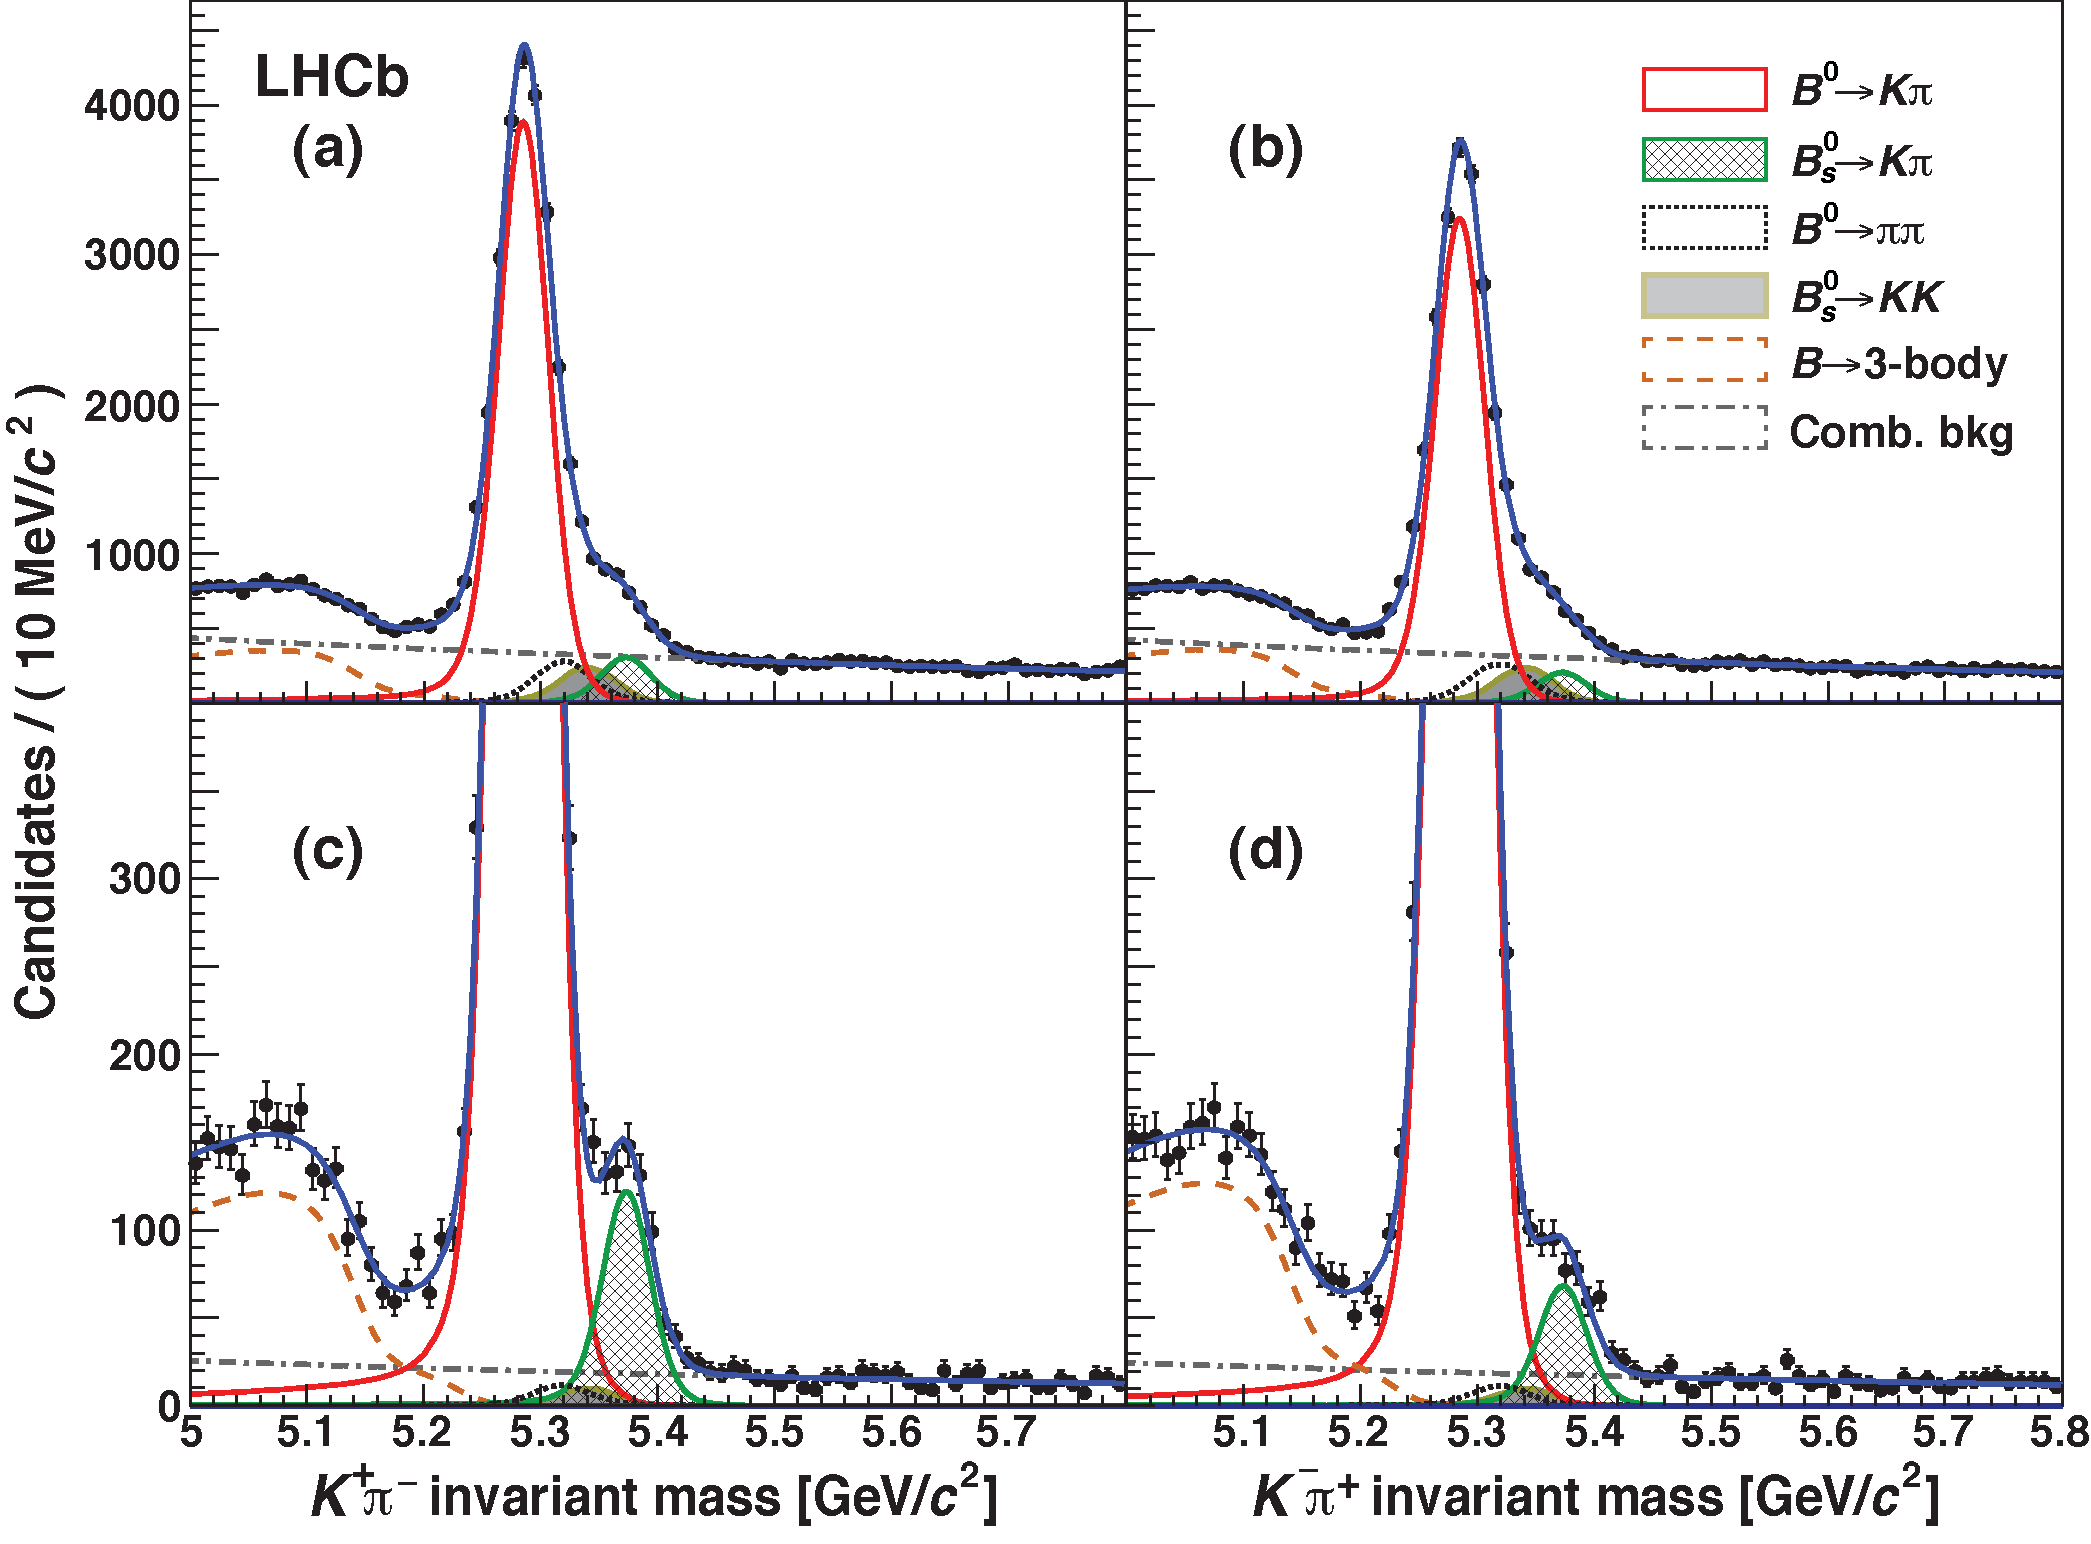
\includegraphics[width=0.8\textwidth]{03CPV/figs/DirectCPV.pdf}
	\caption{Invariant mass spectra for \Bz (top) and \Bs (bottom) decays into \Kp\pim (left) and \Km\pip(right). The result of the unbinned maximum likelihood fits are overlaid~\cite{LHCb-PAPER-2013-018}.}
	\label{fig:DirectCPV}
\end{figure}

\setmathfont[Scale=MatchUppercase]{XITS Math}
\subsection[head={\CP violation in mixing},tocentry={\CP violation in mixing}]{$\symbfsf{C{}P}$ violation in mixing}
\label{sec:MixingCPV}
\setmathfont{Tex Gyre Pagella Math}

Indirect \CP violation, also denoted as \CP violation in mixing, implies that the transition probabilities for a meson \Paz to oscillate into its antiparticle state \Pazb and vice versa are different.
Due to charge conservation, mixing is only possible for uncharged mesons and hence this type of \CP violation cannot occur for charged particles.
Using the time evolution from \cref{eq:timeEvolution}, the probabilities of \eg initially produced \Bz (\Bzb) mesons to have oscillated into a \Bzb (\Bz) at proper-time $t$ are
\begin{align}
\left|\left<\Bz\Big|\Bzb\!\left(t\right)\right>\right|^2=\frac{1}{4}\left|\frac{p}{q}\right|^2
\left(e^{-\GH t}+e^{-\GL t}-2e^{-\Gamma t}\cos\left(\dm t\right)\right)\,,\\
\left|\left<\Bzb\Big|\Bz\!\left(t\right)\right>\right|^2=\frac{1}{4}\left|\frac{q}{p}\right|^2
\left(e^{-\GH t}+e^{-\GL t}-2e^{-\Gamma t}\cos\left(\dm t\right)\right)\,.
\end{align}
To obtain the same probabilities for both processes, the condition
\begin{equation}
\left|\frac{q}{p}\right|=\left|\frac{p}{q}\right| \Rightarrow \left|\frac{q}{p}\right|=1
\end{equation}
has to be satisfied.
According to \cref{eq:qoverp}, this means that indirect \CP violation occurs if the matrix elements $m_{12}$ and $\Gamma_{12}$ have different complex phases.
Using neutral \B mesons as an example, the \CP asymmetry in case of indirect \CP violation is accordingly defined as
\begin{equation}
A_{\CP}=\frac{\Gamma\left(\Bz(t)\!\to\Bzb\right) - \Gamma\left(\Bzb(t)\!\to\Bz\right)}{\Gamma\left(\Bz(t)\!\to\Bzb\right) + \Gamma\left(\Bzb(t)\!\to\Bz\right)}
= \frac{1-\left|\nicefrac{p}{q}\right|^4}{1+\left|\nicefrac{p}{q}\right|^4}\,.
\end{equation}
However, as neutral \B mesons do not just oscillate but also decay this asymmetry cannot be used directly to measure \CP violation in mixing.
Instead, the \B mesons need to be reconstructed in flavour specific decays, \ie only the transitions $\Bz\to\f$ and $\Bzb\to\fbar$, but not $\Bz\to\fbar$ and $\Bzb\to\f$ are allowed.
Thus, the flavour of the meson at decay can be inferred from the final state and compared to the initial production flavour.
For the \Bz and \Bs meson system, \CP violation in mixing has been measured to be negligible \cite{HFLAV2016}, which is in good agreement with the \ac{SM} predictions (see \cref{sec:BBbarMixing}).

\setmathfont[Scale=MatchUppercase]{XITS Math}
\subsection[head={Interference \CP violation},tocentry={Interference \CP violation}]{Interference $\symbfsf{C{}P}$ violation}
\label{sec:InterferenceCPV}
\setmathfont{Tex Gyre Pagella Math}

So far \CP violation arising from a clash between the phases of two interfering decay amplitudes or a clash between the phases of $m_{12}$ and $\Gamma_{12}$ has been discussed.
The third possibility is a clash between the phase of $\nicefrac{q}{p}$ and the phase of the decay amplitude what results in the so-called interference \CP violation.
For this type of \CP violation the initial particle \Paz and antiparticle \Pazb must decay into both the final state \f and its \CP-conjugate \fbar.

Inverting the requirement for \CP violation in mixing shows that \CP is conserved in mixing if there is a phase $\xi'$ such that
\begin{equation}
\begin{split}
m_{12}^\ast &= e^{2i\xi'}m_{12}\,,\\
\Gamma_{12}^\ast &= e^{2i\xi'}\Gamma_{12}\,,\label{eq:CPconservationMixing}
\end{split}
\end{equation}
which leads directly to $\nicefrac{q^2}{p^2} = e^{2i\xi'}$ (\cref{eq:qoverPPurePhase}).
Using \cref{eq:CPTransInitFinal} the \CP conjugated amplitudes \Abarfbar and \Afbar can be expressed as
\begin{align}
\Abarfbar&=e^{i\left(\xi_f-\xi_i\right)}\Af\,\,,\label{eq:amplitudetransformation_1}\\
\Afbar&=e^{i\left(\xi_f+\xi_i\right)}\Abarf\,\,.\label{eq:amplitudetransformation_2}
\end{align}
yielding $\big|\,\Af\,\big|=\big|\,\Abarfbar\,\big|$ and $\big|\,\Abarf\,\big|=\big|\,\Afbar\,\big|$ after eliminating the phases and shows that these amplitudes are not subject to direct \CP violation.
Multiplying \cref{eq:amplitudetransformation_1} and \cref{eq:amplitudetransformation_2} gives the relation
\begin{equation}
\Af\,\Afbar=e^{2i\xi_i}\,\Abarfbar\,\Abarf\,\,.
\end{equation}
Under the assumption that the phase $\xi'$ of $\nicefrac{q}{p}$ and the \emph{weak} phase $\xi_i$ are the same, one finds \CP conservation and
\begin{equation}
\arg\left(\frac{p^2}{q^2}\Af \,\overline{\kern -1.0pt A\kern -1.0pt}_{\kern 1.0pt f}^\ast\,\Afbar\overline{\kern -1.0pt \,A\kern -1.0pt}_{\kern 2.5pt\overline{\kern -1.5pt f\kern 1.5pt}}^\ast\right)=0
\end{equation}
applies.
However, $\xi_i=\xi'$ is a very specific case and thus even without the presence of \CP violation in decay or mixing, \CP is not conserved.
This also can be expressed using the parameters \Lf and \Lfbar.
In the case of \CP conservation in decay or mixing $\big|\Lf\big|=\big|\Lfbar\big| = \pm1$) holds while \CP is not conserved in case of
\begin{equation}
	\arg\left(\Lf\right)+\arg\left(\Lfbar\right)\neq0\,. \label{eq:conditionCPV}
\end{equation}
This means the \CP coefficients \Cf and \Cfbar are not affected by this type of \CP violation, while for the coefficients $(\Sf, \Sfbar)$ and  ($A_f^{\DG}, A_{\kern 1.5pt\overline{\kern -1.5pt f\kern 1.5pt}}^{\DG})$ this condition can be reformulated to
\begin{equation}
\Sf\neq-\Sfbar\,\,\,\,\,\text{and}\,\,\,\,\,A_f^{\DG}\neq A_{\kern 1.5pt\overline{\kern -1.5pt f\kern 1.5pt}}^{\DG}\,.\label{eq:condForIntCPV}
\end{equation}
In case that both, particle and antiparticle, decay into only one common final state this conditions simplifies to $\arg\left(\Lf\right)\neq0$ and $\Sf\neq0$, $A_f^{\DG}\neq0$.

\CP violation in the interference of decay and decay after mixing was first observed by the \B-factories \babar \cite{Aubert:2001nu} and \belle \cite{Abe:2001xe} in the so-called golden mode \BdToJPsiKS.
This measurement is the most prominent one for this type of \CP violation allowing to determine $\sin\!\left(2\beta\right)$.
For \BdToJPsiKS no \CP violation in decay and mixing is expected and with the current experimental precision $\DG=0$ can be assumed.
Therefore, the \CP asymmetry in this case can be expressed as
\begin{equation}
A_{\CP}(t)=\frac{\Gamma\left(\Bzb\to\jpsi\KS\right)-\Gamma\left(\BdToJPsiKS\right)}{\Gamma\left(\Bzb\to\jpsi\KS\right)+\Gamma\left(\BdToJPsiKS\right)}\approx\Sf\sin\left(\dmd t\right)\label{eq:CPAsymBd2JpsiKS}
\end{equation}
where the parameter \Sf can be identified with $\sin{}\left(2\beta\right)$.
The most recent measurement of \Sf was performed by \lhcb \cite{Aaij:2015vza} yielding a result of
\begin{equation}
\Sf=0.731\pm0.035\stat\pm0.005\syst\,,
\end{equation}
and is consistent with the \ac{SM} expectation. The resulting time-dependent signal yield asymmetry is shown in \cref{fig:sin2beta}
\begin{figure}[tb]
	\centering
	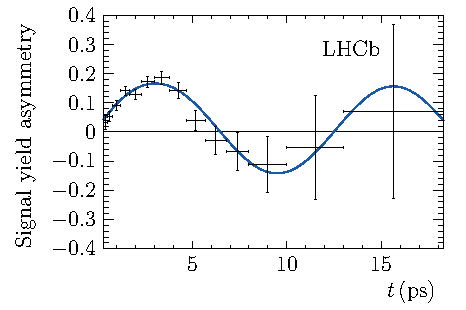
\includegraphics[width=0.6\textwidth]{03CPV/figs/InterferenceCPV.pdf}
	\caption{Time-dependent signal yield asymmetry $\left(N_{\Bzb}-N_{\Bz}\right)/\left(N_{\Bzb}+N_{\Bz}\right)$ for the decay \BdToJPsiKS.
	The black points represent the data sample, the blue solid curve is the projection of the signal \PDF~\cite{Aaij:2015vza}.}
	\label{fig:sin2beta}
\end{figure}
